\documentclass[11pt]{article}
\usepackage[T1]{fontenc}
\usepackage[utf8]{inputenc}
\usepackage[margin=2cm]{geometry}
\usepackage{amsmath,amssymb,booktabs,longtable,array}
\usepackage{tikz}
\usetikzlibrary{arrows.meta,positioning,shapes.geometric}
\usepackage{listings}
\usepackage[hidelinks]{hyperref}
\lstset{basicstyle=\ttfamily\footnotesize,columns=fullflexible,keepspaces=true,
  breaklines=true,breakatwhitespace=false,showstringspaces=false,
  frame=single,aboveskip=0.8em,belowskip=0.8em}
\newcommand{\code}[1]{\texttt{#1}}
\tikzset{box/.style={draw,rounded corners,align=center,text width=3.1cm,
  minimum height=1cm,font=\small,fill=blue!4},
  outer/.style={box,fill=gray!10},
  flow/.style={-{Latex},thick},
  lab/.style={font=\scriptsize,align=center,fill=white,inner sep=2pt}}
\title{FunSearch pack v1: design and operating contract\\[0.5em]
  \large Status: as designed (2026-10-05); refreshed at epic close-out}
\author{Math City / FunSearch pack}
\date{2026-10-05}
\begin{document}
\maketitle
\noindent This article records the decisions in the authoritative DESIGN field of
Gas City epic \code{mc-h4zx}, designed by kurt with the overseer on 2026-10-05.
It is a design record; the close-out bead refreshes it against the implementation.
The epic DESIGN wins if a child bead disagrees, and real conflicts are recorded
on that bead. This document does not gate implementation work.
\tableofcontents

\section{Overview}
The \code{funsearch} Gas City pack orchestrates evolutionary program search in the
FunSearch / AlphaEvolve lineage \cite{funsearch,alphaevolve,ellenberg,kitft}.
A user supplies a problem directory and an evaluator with a C interface.
The pack supplies the engine, worker, and mutator agent role. All problem
knowledge belongs to the evaluator; the pack works in any rig.

New candidate programs are whole source files written by a small coding agent,
rather than a single model completion. This is the agentic variation operator
pattern \cite{avo}: a mutator reads parents and feedback, writes a child,
and can compile and test it before submitting. Authoritative scoring still
belongs to the engine and evaluator.

The design trades sample volume for effort per child. The intended comparison
is FunSearch at roughly millions of samples, AlphaEvolve at thousands, and this
pack at hundreds. These are order-of-magnitude planning estimates, not comparable
benchmark measurements or results of our acceptance run. The epic expects about
50--100 times fewer samples than FunSearch, with better prepared candidates.
The acceptance run measures throughput and validity to test that expectation.
Related work includes sample-efficient evolution \cite{shinka} and analysis of
what evolutionary coding agents evolve \cite{agents-evolve}.

\subsection{Repository, licensing, and portability}
The public pack repository is \url{https://github.com/jjgarzella/funsearch-pack},
licensed Apache-2.0. It is a submodule at \code{packs/funsearch} in Math City
(the deployment path is
\path{/home/jjgarzella/Developer/ai/city/math-city/packs/funsearch}).
\code{pack.toml} names the pack \code{funsearch} and uses schema 2, following
\code{packs/labtech/pack.toml}. There are no required rig-specific formula
variables or hard-coded rig names or paths in the pack. If code is copied or
adapted from \code{kitft/funsearch}, add an Apache-2.0 NOTICE crediting it.

\section{Glossary}
The following twelve definitions reproduce design section 3 exactly; these
terms are used in code, documentation, and prompts.
\small
\begin{longtable}{@{}p{1.7cm}p{14.8cm}@{}}
\toprule Term & Meaning \\ \midrule
\endfirsthead
\toprule Term & Meaning \\ \midrule
\endhead
\textbf{problem} & A directory, anywhere on disk, that fully describes one search problem. Passed to a run as a path. Lives in whatever rig uses it, never in the pack (except the bundled example). \\
\textbf{instance} & An opaque string of \texttt{key=value} pairs separated by commas, e.g. \texttt{n=6} or \texttt{q=5,d=3}. There is exactly ONE per run. The engine never parses it. It is passed unchanged to \texttt{fs\_init} and \texttt{fs\_score}. \\
\textbf{candidate} & One evolved program: a whole source file (default language C) that must export the symbols declared in the problem's \texttt{candidate.h}. It may contain any helpers or static data. \\
\textbf{evaluator} & A user-supplied shared library with a C interface that scores a candidate. It is entirely the problem author's code; all problem knowledge lives here. It can be written in any language, e.g. C embedding Julia. \\
\textbf{result} & What \texttt{fs\_score} returns: status + score + optional signature + message. \\
\textbf{score} & A \texttt{double}, higher is better. Only meaningful when status is \texttt{FS\_OK}. \\
\textbf{signature} & Up to 8 doubles describing a candidate's behaviour. Used ONLY for grouping candidates within an island and for duplicate rejection, never for ranking. \\
\textbf{worker} & A small C host process supplied by the pack (\texttt{funsearch-worker}). It loads the evaluator once, then scores candidates one at a time. \\
\textbf{engine} & A Python 3 + SQLite program supplied by the pack. It runs one run: the program database, islands, task issuing, compile → score pipeline, stop conditions and CLI. \\
\textbf{mutator} & The pack's agent role. It writes child candidates by looping \texttt{next-task} → write → \texttt{try} → \texttt{submit}. \\
\textbf{run} & One engine execution on one problem + one instance + one config. It has a run directory and a run bead. \\
\textbf{slot bead} & One of K beads per run, routed to the mutator pool. Each represents one concurrent mutator seat. \\
\bottomrule
\end{longtable}
\normalsize

\section{Architecture flowchart}
\begin{figure}[htbp]
\centering
\resizebox{\linewidth}{!}{%
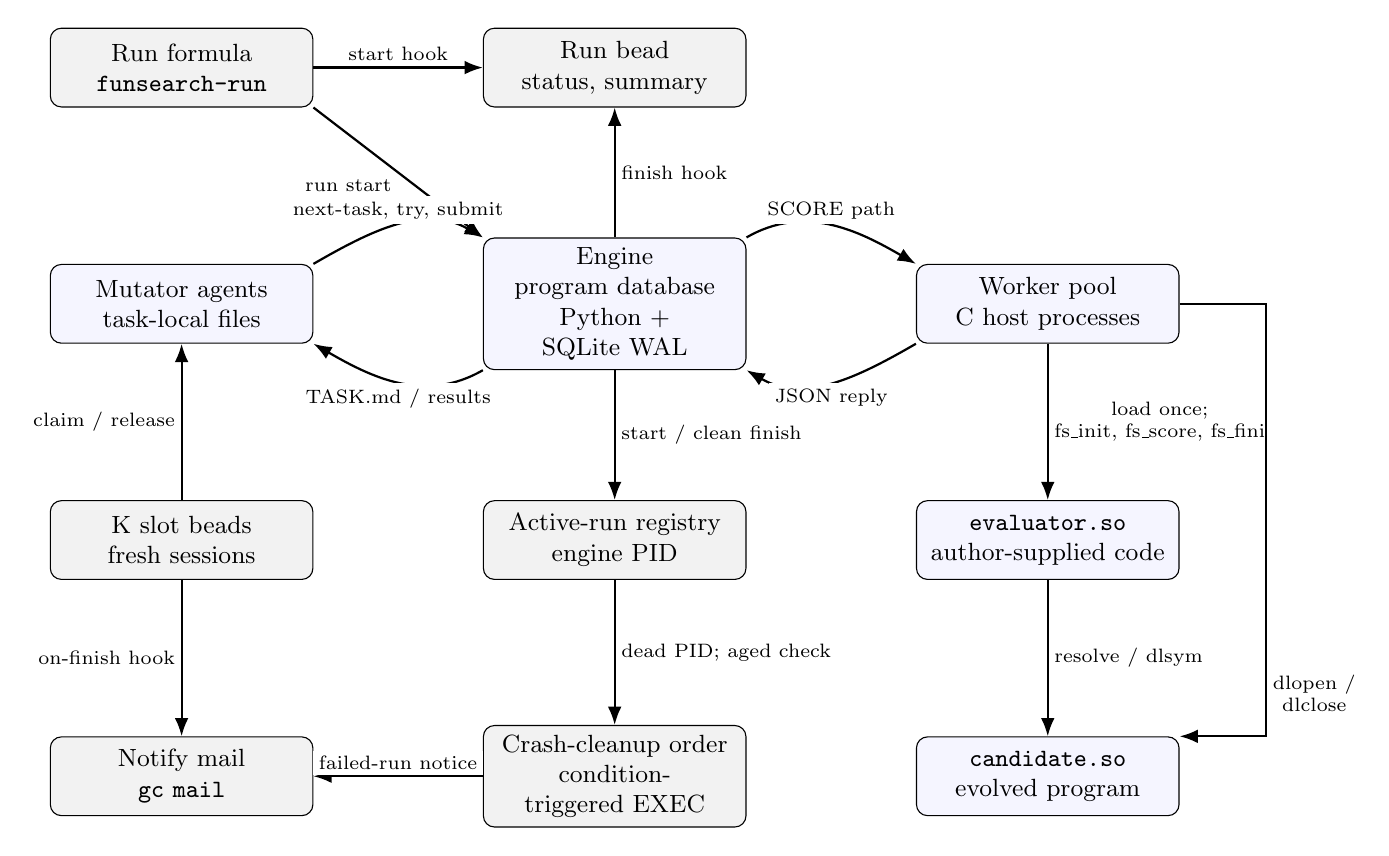
\begin{tikzpicture}
\node[outer] (formula) at (0,3) {Run formula\\\code{funsearch-run}};
\node[outer] (run) at (5.5,3) {Run bead\\status, summary};
\node[box] (mutator) at (0,0) {Mutator agents\\task-local files};
\node[box] (engine) at (5.5,0) {Engine\\program database\\Python + SQLite WAL};
\node[box] (worker) at (11,0) {Worker pool\\C host processes};
\node[outer] (slots) at (0,-3) {K slot beads\\fresh sessions};
\node[outer] (registry) at (5.5,-3) {Active-run registry\\engine PID};
\node[box] (evaluator) at (11,-3) {\code{evaluator.so}\\author-supplied code};
\node[outer] (mail) at (0,-6) {Notify mail\\\code{gc mail}};
\node[outer] (sweep) at (5.5,-6) {Crash-cleanup order\\condition-triggered EXEC};
\node[box] (candidate) at (11,-6) {\code{candidate.so}\\evolved program};
\draw[flow] (formula) -- node[lab,above] {start hook} (run);
\draw[flow] (formula.south east) -- node[lab,below left] {run start} (engine.north west);
\draw[flow] (engine) -- node[lab,right] {finish hook} (run);
\draw[flow] (mutator.north east) to[out=30,in=150] node[lab,above] {next-task, try, submit} (engine.north west);
\draw[flow] (engine.south west) to[out=210,in=330] node[lab,below] {TASK.md / results} (mutator.south east);
\draw[flow] (engine.north east) to[out=30,in=150] node[lab,above] {SCORE path} (worker.north west);
\draw[flow] (worker.south west) to[out=210,in=330] node[lab,below] {JSON reply} (engine.south east);
\draw[flow] (worker) -- node[lab,right] {load once;\\fs\_init, fs\_score, fs\_fini} (evaluator);
\draw[flow] (evaluator) -- node[lab,right] {resolve / dlsym} (candidate);
\draw[flow] (worker.east) -- ++(1.1,0) |- node[lab,pos=0.45,right] {dlopen /\\dlclose} (candidate.north east);
\draw[flow] (slots) -- node[lab,left] {claim / release} (mutator);
\draw[flow] (engine) -- node[lab,right] {start / clean finish} (registry);
\draw[flow] (registry) -- node[lab,right] {dead PID; aged check} (sweep);
\draw[flow] (sweep) -- node[lab,above] {failed-run notice} (mail);
\draw[flow] (slots) -- node[lab,left] {on-finish hook} (mail);
\end{tikzpicture}}
\caption{Core search and outer Gas City lifecycle. CLI processes and the daemon
communicate only through SQLite. The engine core never calls \code{gc}; hook
scripts create/close beads and mail. The sweep also closes stranded slot beads.}
\label{fig:architecture}
\end{figure}
The worker loads each candidate, supplies a resolver bound to that candidate's
handle, and lets the evaluator call the required candidate symbols. The
signature groups behaviour and rejects duplicates; it never ranks candidates.
The mutator's reported score is never authoritative. Outer arrows summarize hook-managed bookkeeping, rather than
direct bead-to-bead communication.

\section{Run life cycle}
\begin{enumerate}
\item An experimenter prepares a problem and uses \code{check} for pre-flight.
The thin run formula starts a run with its instance, optional overrides and
notification recipient. The engine validates the problem, builds the evaluator,
and requires the compiled seed to score \code{FS\_OK}.
\item The engine creates a run directory, daemonizes, and prints its ID and path.
The start hook receives that path, creates the run bead and K raw-routed slot
beads, and registers the engine PID in the city's active-run registry.
\item Each fresh mutator session claims a slot and performs N tasks:
\code{next-task} $\to$ write \code{child.c} $\to$ bounded \code{try} $\to$
\code{submit}. After N tasks it releases the still-routed, unassigned, open
slot bead and exits; another fresh session takes the seat. A duplicate submission
does not consume the task, so the mutator must revise and submit again.
\item The engine keeps scoring and evolving until duration, maximum children,
plateau, or an explicit \code{stop} ends the run. \code{next-task} then reports
\code{RUN\_OVER}, exiting 3, and mutators close their slots.
\item At stop the engine writes \code{summary.json}, exports \code{best.c} and
\code{top/<k>.c}, backs up SQLite, and stops workers. It invokes the finish hook
with the run directory and \code{FS\_RUN\_DIR} set, then exits.
\item The finish hook updates the run bead with its summary, closes it and any
remaining slot beads, mails the \code{notify} recipient, and deletes the registry
entry. No result or source is automatically committed.
\item If the engine dies before clean finish, the dormant condition-triggered
sweep runs only with active entries and a last-sweep age greater than 30 minutes.
For each dead PID it marks the run failed using the last summary or snapshot,
closes its slots, mails notify, and removes the entry; it updates the sweep timestamp.
\end{enumerate}
This sequence separates normal completion, which the engine owns, from crash
recovery, which the EXEC order owns. N controls context recycling; K controls
concurrent mutator seats. Each slot incurs one bead write per N mutations,
acceptable at roughly 100 mutations per hour.

\section{Problem directory and configuration}
A problem may live anywhere on disk. Except for the bundled example it lives in
the rig that uses it, never in the pack. The mutator receives a task-local
presentation rather than direct access to this directory.
\begin{lstlisting}
<problem>/
  problem.toml    # config (below)
  problem.md      # the maths in prose: goal, what is known, hints. This is what the mutator reads.
  candidate.h     # exact C prototypes the candidate must export, with comments
  seed.c          # the starting candidate, usually trivial
  evaluator/      # evaluator source + build script (or a prebuilt .so)
  runs/           # created by the engine, gitignored: one subdirectory per run
\end{lstlisting}
The v1 \code{problem.toml} schema below is copied verbatim, including comments,
from the epic. The instance is opaque to the engine: exactly one is used for a
run, and it is passed unchanged to \code{fs\_init} and \code{fs\_score}. A run can
override \code{instance}, \code{[search]}, and \code{[stop]} keys on the command line.
\begin{lstlisting}
[problem]
name = "cap-set"
instance = "n=6"                 # default instance, overridable per run

[candidate]
language = "c"
compile = "cc -O2 -shared -fPIC -o {out} {src}"          # {src}, {out} substituted
compile_try = "cc -O1 -g -fsanitize=address,undefined -shared -fPIC -o {out} {src}"  # for `try`
exports = ["priority"]           # symbols that must be present in the .so (checked with nm / dlsym)

[evaluator]
build = "make -C evaluator"      # run once at run start in the problem dir; may be empty
library = "evaluator/libevaluator.so"
timeout_s = 30                   # per fs_score call
memory_mb = 2048                 # RLIMIT_AS for the worker

[search]
islands = 4
mutators = 3                     # K = number of slot beads
tasks_per_session = 1            # N: tasks a mutator session handles before recycling
trial_budget = 3                 # max `try` calls per task
parents_per_task = 2
workers = 2                      # worker processes
reset_period_s = 1800            # weakest-half island reset period

[stop]
duration_s = 3600
max_children = 100
plateau_children = 0             # 0 = disabled; else stop after this many children with no improvement

[mutator]
model = "claude-haiku-4-5-20251001"
\end{lstlisting}
The normal compiler is used for authoritative submission; \code{compile\_try}
adds sanitizers for trial evaluation. The configured exports must be present
in the resulting library, checked with \code{nm} / \code{dlsym}.

\section{Evaluator C contract and author rules}
The following is the verbatim design-section-5 contract for the pack's
\code{include/funsearch.h}. An evaluator can use any implementation language
behind this ABI, including a C wrapper embedding Julia.
\begin{lstlisting}[language=C]
typedef enum { FS_OK = 0, FS_INVALID = 1, FS_ERROR = 2 } fs_status;
typedef struct {
  fs_status status;
  double    score;      /* higher is better; meaningful only if FS_OK */
  int32_t   nsig;       /* 0..8 */
  double    sig[8];
  char      msg[256];   /* shown to the mutator during `try`; NUL-terminated */
} fs_result;

/* resolve(sym) returns the address of symbol `sym` in the candidate, or NULL. */
typedef void *(*fs_resolve_fn)(const char *sym);

/* REQUIRED */
fs_result fs_score(fs_resolve_fn resolve, const char *instance);
/* OPTIONAL: called once per worker process before any fs_score / at shutdown. */
int  fs_init(const char *instance);   /* nonzero = fatal: the run fails at startup */
void fs_fini(void);
\end{lstlisting}
\begin{itemize}
\item Never return \code{FS\_OK} without independently checking the object the
candidate produced. That check must not call the candidate.
\item Use exact or interval arithmetic where floating-point errors could be exploited.
\item Explicitly reject degenerate outputs with \code{FS\_INVALID} and a clear
\code{msg}. The verifier-loophole lesson motivates this responsibility
\cite{exploration}.
\item Internal structure---multiple sizes, a cheap-first cascade, or early exit---is
the evaluator's business. Return one score; per-size values may appear in \code{sig}.
\end{itemize}
Scores are higher-is-better doubles and meaningful only for \code{FS\_OK}.
Signatures contain at most eight doubles. The status distinguishes invalid
objects from evaluation errors, while the NUL-terminated message explains feedback
to the mutator during trials.

\section{Worker protocol}
\code{funsearch-worker <evaluator.so> <instance>} loads the evaluator once.
If present, \code{fs\_init} runs before any score call; a nonzero result prints
an error line and exits 3, failing run startup.

There is one request per stdin line and one JSON result per stdout line:
\begin{lstlisting}
SCORE <absolute path to candidate .so>
{"status":"OK|INVALID|ERROR","score":<num>,"sig":[...],"msg":"..."}
QUIT
\end{lstlisting}
For each SCORE request, the worker opens the candidate using
\code{dlopen} with flags \code{RTLD\_NOW|RTLD\_LOCAL}, binds a resolve function to
\code{dlsym} on that handle, calls \code{fs\_score}, then \code{dlclose}s it.
The worker evaluates one candidate at a time. On \code{QUIT}, it calls
\code{fs\_fini} if present and exits 0.

The engine owns timeouts and crash handling: it kills the worker on timeout,
records \code{ERROR} with ``timeout'' or ``worker crashed: signal N'', and
starts a replacement worker. If \code{FS\_MEMORY\_MB} is set, the worker uses its value to apply the
\code{RLIMIT\_AS} memory limit through \code{setrlimit}. It must not install SIGSEGV handlers:
embedded Julia uses its own. A warm evaluator process is therefore reused across
candidates, while each candidate library has a per-request lifetime.

\section{Engine: CLI, database, and evolution}
The engine uses Python 3's standard library and SQLite, without third-party
Python dependencies. Its entry point is \code{bin/funsearch}.
\subsection{Command-line contract}
\begin{lstlisting}
funsearch check <problem> [--instance S]
funsearch run start <problem> [--instance S] [--run-id ID]
    [--set key=val ...] [--on-start CMD] [--on-finish CMD]
funsearch run status <run-dir>
funsearch best <run-dir> [-k N]
funsearch stop <run-dir>
funsearch next-task <run-dir> [--slot ID]
funsearch try <run-dir> <task-id> <candidate.c>
funsearch submit <run-dir> <task-id> <candidate.c>
funsearch rescore <run-dir> <program-id|best> --instance S
\end{lstlisting}
\begin{description}
\item[check] Validates the directory and TOML, builds the evaluator, compiles the
seed, scores it with a fresh worker, and prints the result. It performs no search.
\item[run start] Performs pre-flight (seed must score \code{FS\_OK}), creates the
run directory, and daemonizes the loop. It prints the run ID and directory.
Optional start/finish hook commands receive the run directory as their only
argument, with \code{FS\_RUN\_DIR} also set. The engine itself never calls \code{gc}.
\item[run status / best / stop] Inspect the run, retrieve the best programs
(optionally top N), or request engine-owned termination.
\item[next-task] Prints a task ID and directory containing \code{TASK.md}:
\code{problem.md}, \code{candidate.h}, scored parents and messages, a short
``already tried'' summary, trial budget, and instructions. If stopped it prints
\code{RUN\_OVER} and exits 3.
\item[try] Compiles with \code{compile\_try}, scores through the daemon's worker
pool, and prints the result. It refuses calls once that task's trial budget is used.
\item[submit] Normalizes and hashes code, rejects exact and normalized duplicates,
and rejects a child whose signature and score equal an existing program's.
Rejection does not consume the task. Otherwise it compiles with \code{compile},
scores authoritatively (ignoring any mutator-reported score), stores the child,
and closes the task.
\item[rescore] Uses a temporary worker to score a stored program on another
instance; the original run still has its single instance.
\end{description}
\subsection{Storage and evolutionary policy}
The program database is \code{<run-dir>/db.sqlite} in WAL mode. It stores programs
(ID, parent IDs, island, source, normalized hash, status, score, signature,
message, timestamps), tasks, trials, an evaluation queue, and run state.
The daemon owns the worker pool and handles queued trial/submission evaluations.
CLI processes and the daemon communicate only through SQLite.

Evolution follows FunSearch / kitft: maintain islands, grouping programs within
an island in clusters keyed by (score, signature). Sample parents using a
Boltzmann distribution over cluster scores, with temperature decreasing as the
island grows; prefer shorter programs within a cluster. Periodically reset the
weakest half of islands, reseeding them from the best programs of the survivors.
Signatures are grouping and duplicate-rejection information, never a ranking
objective; score alone determines quality.

\subsection{Stop and durable output}
The engine owns duration, \code{max\_children}, plateau, and explicit-stop
conditions. \code{plateau\_children = 0} disables plateau stopping; otherwise
stop after that many children without improvement. On stopping, it writes
\code{summary.json}, exports \code{best.c} and \code{top/<k>.c}, shuts down
workers, runs the finish hook, and exits. Periodic snapshots and the final
snapshot copy SQLite using its backup API.

\section{Mutator role}
The pack's \code{agents/mutator/} role uses provider \code{claude}, default model
\code{claude-haiku-4-5-20251001}; the problem's \code{[mutator] model} can override
it. It is a pool with \code{max\_active\_sessions} large enough for K (default 3)
and \code{wake\_mode} fresh.

Allowed tools are shell only for the pack's \code{funsearch next-task|try|submit}
and file reads/writes only inside the task directory. No web, git, direct
problem-directory reads, or evaluator-source reads are allowed. The slot
bootstrap claims its routed bead using \code{gc hook --claim}; run directory
and slot ID come from metadata. These lifecycle bead operations accompany the
restricted mutation loop, rather than giving general shell access.

The session repeats N times: obtain a task, write a child, try at most the
budget, and submit. It releases the slot back to the queue after N tasks,
keeping it routed, unassigned, and open, then exits for clean-context recycling.
On \code{RUN\_OVER}, it closes the slot and exits.

\section{Gas City integration}
\subsection{Formula and beads}
The thin \code{funsearch-run} formula has variables \code{problem}, optional
\code{instance}, \code{notify} (default the slinger), and optional
\code{overrides}. Its single step executes \code{funsearch run start ...}
and records the outcome. Slot beads are routed raw with \code{--no-formula}
to \code{<rig>/funsearch.mutator}; they use no review/PR formula.

Each run has one run bead in its starting rig, labelled \code{funsearch-run}.
Its metadata includes problem, run directory, instance, engine PID, status,
best score, children scored, and notify. Its final summary note records best
score, \code{best.c} path, throughput, and fraction of children scoring OK.
The active registry at \code{<city>/.gc/funsearch/active/<run-id>.json} is
written at start and deleted after a clean finish.

\subsection{Completion and crash sweep}
The engine finishes its own runs through the finish hook: update and close the
run bead, close any remaining slots, and send \code{gc mail} to notify. This is
mail, not a nudge.

\code{funsearch-sweep} is a condition-triggered EXEC order, with no agent.
Its check exits 0 only when the active directory is nonempty and the timestamp
of the last sweep is more than 30 minutes old. For each registered run with a
dead engine PID, the script marks the run bead failed with the latest summary
or snapshot information, closes slots, mails notify, removes the registry file,
and updates the timestamp. It remains dormant without active runs. Run
directories are gitignored, and nothing is committed automatically.

\section{Cap-set example and acceptance}
The bundled problem lives at \code{examples/cap-set/}. Its candidate ABI is
\begin{lstlisting}[language=C]
double priority(const int8_t *v, int32_t n);
\end{lstlisting}
Here \code{v} has length n, with entries in $\{0,1,2\}$. The evaluator is a C
wrapper embedding Julia (libjulia). Its \code{fs\_init} starts Julia once and
loads \code{capset.jl}. Its \code{fs\_score} calls a Julia greedy construction
that \code{ccall}s the resolved priority pointer, then independently checks that
the produced set is a cap set. For distinct $x,y,z\in\mathbb{F}_3^n$, the
forbidden condition is
\[
 x+y+z\equiv 0\pmod 3.
\]
The verifier does not call the candidate. Score is the cap size $|C|$ at n
from the instance (default \code{n=6}), and the signature contains cap sizes
at $n=4,5,6$. The seed returns constant priority. The design records known
optimum sizes $2,4,9,20,45,112$ for $n=1,\ldots,6$.

The acceptance bead runs in rig \code{math-experiments}, with 3 mutators,
for about one hour or 100 children. It passes when the run completes unattended,
the best score strictly exceeds the seed score, and every recorded cap passes
an independent re-check. It reports throughput, share of children scoring OK,
session startup cost, and a recommended N (tasks per session). These are future
acceptance criteria, not results claimed by this design document.

\section{Local landing and epic close-out}
All implementation beads land on the pack's local \code{main}. Nothing is
pushed until the close-out bead. Each bead creates a worktree on
\code{fs/<bead>} off local main, implements, runs its acceptance commands,
rebases, fast-forwards the pack's main, removes the worktree/branch, records
results, closes the bead, and dispatches ready successors. Beads labelled
\code{fs-manual} are never auto-dispatched. This documentation bead changes
only the pack, not the Math City repository.

The final review is one \code{mol-review-loop-standard} pass over
\code{origin/main..funsearch-v1}. After convergence, the authorized close-out
pushes \code{funsearch-v1:main} and bumps only the relevant submodule-pointer
and Math City import lines. The overseer waived the human merge gate for this
epic. The design document is refreshed at close-out to match what was built.

\section{Decision log: Q1--Q24}
The epic records the resolved design, not the original interview transcript.
Except for the supplied Q16 example, the Q labels below are a reconstruction
for this record, derived from the design; they do not claim original question wording.
\begin{enumerate}
\renewcommand{\labelenumi}{Q\arabic{enumi}:}
\item Package the search as a project-agnostic Gas City pack named \code{funsearch}.
\item Use an agentic mutator that writes, compiles, and tests whole candidates.
\item Trade sample volume for per-child quality; plan for hundreds of children.
\item Publish an Apache-2.0 pack submodule and credit any kitft-derived code in NOTICE.
\item Keep each problem self-contained in a directory owned by its using rig.
\item Use exactly one opaque instance string per run, passed unchanged through the ABI.
\item Start with C candidates exporting the problem's \code{candidate.h} symbols.
\item Put all problem knowledge in a user-supplied shared evaluator with a C ABI.
\item Return status, one higher-is-better double score, optional signature, and message.
\item Use at most eight signature doubles for clustering and duplicates, never ranking.
\item Require independent validation, exact/interval checks, and explicit invalid-output rejection.
\item Reuse a C worker's evaluator, resolving and unloading each candidate per request.
\item Let the engine replace timed-out/crashed workers; apply RLIMIT\_AS and no SIGSEGV handler.
\item Use a dependency-free Python/SQLite WAL engine, with queue-only CLI/daemon communication.
\item Own normal stopping in the engine and export summaries, best code, and backup-API snapshots.
\item The engine finishes its own runs; a dormant condition-triggered EXEC order sweeps crashes every $\geq$30 minutes (the check requires more than 30 minutes since the last sweep).
\item Evolve islands using (score, signature) clusters, Boltzmann parent sampling, shorter-code preference, and weakest-half resets.
\item Offer pre-flight, start/status/best/stop, next-task/try/submit, and alternate-instance rescore commands.
\item Bound trials per task, rescore submissions authoritatively, and reject duplicates without consuming tasks.
\item Restrict mutators to task-local files and search commands, defaulting to Claude Haiku with a problem override.
\item Represent K concurrent seats by raw-routed slot beads and recycle fresh sessions after N tasks.
\item Keep Gas City outside engine core: thin run formula, lifecycle hooks, registry, run bead, and completion mail.
\item Bundle the Julia-backed cap-set problem; require unattended improvement, independent rechecks, and throughput/startup measurements.
\item Land locally through per-bead worktrees, run one whole-epic review, then push and refresh documentation at close-out.
\end{enumerate}

\section{Out of scope and backlog}
The backlog epic holds analysis/generalization agents; an AEvo-style supervising
agent; bandit model ensembles; a one-shot API sampler tier; worker network
isolation; candidate languages other than C (overridable via TOML but untested);
multi-objective scoring; and an interactive problem-setup agent.

\begin{thebibliography}{9}
\raggedright
\bibitem{funsearch} B. Romera-Paredes et al.
\emph{Mathematical discoveries from program search with large language models}.
Nature, published 2023.
\url{https://www.nature.com/articles/s41586-023-06924-6}.
\bibitem{ellenberg} J. S. Ellenberg et al.
\emph{Generative Modeling for Mathematical Discovery}. 2025.
\url{https://arxiv.org/abs/2503.11061}.
\bibitem{kitft} kitft/funsearch. \emph{Genetic programming using LLMs}.
Apache-2.0 implementation. \url{https://github.com/kitft/funsearch}.
\bibitem{alphaevolve} Google DeepMind.
\emph{AlphaEvolve: A Gemini-powered coding agent for designing advanced algorithms}.
2025. \url{https://deepmind.google/blog/alphaevolve-a-gemini-powered-coding-agent-for-designing-advanced-algorithms/}.
\bibitem{exploration} B. Georgiev, J. G\'omez-Serrano, T. Tao, and A. Z. Wagner.
\emph{Mathematical exploration and discovery at scale}. 2025.
\url{https://arxiv.org/abs/2511.02864}.
\bibitem{avo} T. Chen et al.
\emph{AVO: Agentic Variation Operators for Autonomous Evolutionary Search}. 2026.
\url{https://arxiv.org/abs/2603.24517}.
\bibitem{shinka} R. T. Lange, Y. Imajuku, and E. Cetin.
\emph{ShinkaEvolve: Towards Open-Ended And Sample-Efficient Program Evolution}.
2025. \url{https://arxiv.org/abs/2509.19349}.
\bibitem{agents-evolve} \emph{What Do Evolutionary Coding Agents Evolve?} 2026.
\url{https://arxiv.org/abs/2605.20086}.
\end{thebibliography}
\end{document}
